\documentclass[a4paper,12pt]{article}
\usepackage[utf8x]{inputenc}
\usepackage[spanish]{babel}
\usepackage{amsmath}
\usepackage{graphicx}
\usepackage{wrapfig}
\setlength{\textheight}{235mm}
\setlength{\textwidth}{168mm}
\setlength{\oddsidemargin}{0pt}
\pagestyle{empty}

\begin{document}
\mbox{}\vspace*{-45mm}

{\centering
{\small\sc 
%Escuela Técnica Superior de Ingenieros de Caminos, Canales y Puertos (Madrid)\\*[4mm]
Máster Universitario en Ingeniería de Estructuras, Cimentaciones y Materiales}\\*[4mm]
{\Large\bf Método de los Elementos Finitos 24-25}\\*[4mm]
PRÁCTICA 2: Modelos de difusión \\*[4mm]
}

\vspace{3mm}



\begin{wrapfigure}[18]{r}[5mm]{90mm}
\begin{center}
 \vspace{-30pt}
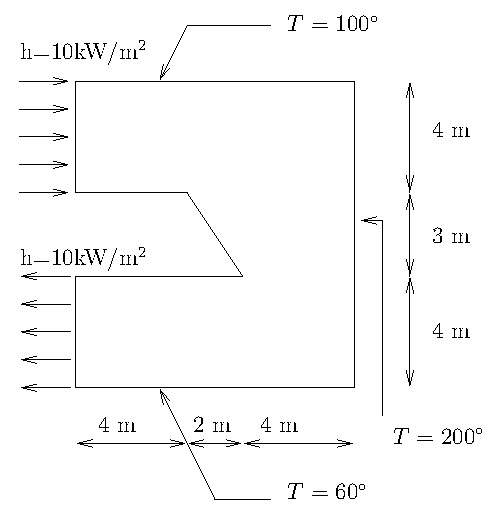
\includegraphics[width=90mm]{practi4}
\end{center}
\end{wrapfigure}

Se considera una chapa cuyas dimensiones y geometría son las indicadas
en la figura adjunta. Los lados de la chapa tienen condiciones de contorno 
correspondientes a temperaturas o flujos impuestos, cuyos valores
también están indicados en dicha figura. Los bordes en los que no se indica
el flujo o la temperatura impuesta se supone que están térmicamente aislados.
El coeficiente de conductividad térmica es $\lambda=1417.4$ W/(m$\cdot$C).\\

Se usarán preferentemente elementos cuadriláteros (\emph{Quad dominated}) para la creación de la malla y la técnica de mallado \emph{Free}, con tamaño global de malla 0.5 m. e interpolación lineal (Elemento \emph{DC2D4}).\\


Se pide:
\begin{itemize}
\item Conocer la distribución de temperaturas y el flujo de calor en la chapa.

\item Repetir el problema considerando dos materiales diferentes. El primero (parte superior con altura de 4m) tiene el mismo coeficiente de conductividad anterior; mientras que el resto de la parte inferior tiene $\lambda=932.5$ W/(m$\cdot$C) 
\end{itemize}

\end{document}

\vspace{3mm}

\hspace{20mm}\hrulefill$\star$\hrulefill\hspace{20mm}

\vspace{3mm}

Resultado del ejercicio con dos materiales:

\begin{itemize}
\item
\end{itemize}

\end{document}
